\documentclass[8pt]{beamer}
\usetheme{Antibes}
\useinnertheme{rectangles}
\useoutertheme{infolines}
\usepackage[utf8]{inputenc}
\usepackage[T1]{fontenc}
\usepackage[ngerman]{babel}

% Patch the look of +, = in arev
\usefonttheme{serif} 

\usepackage{arev}
\usepackage{amsmath}
\usepackage{amssymb}
\usepackage{booktabs}

% Patch punctuation to be upright
\DeclareMathSymbol{.}{\mathpunct}{operators}{`.}
\DeclareMathSymbol{,}{\mathpunct}{operators}{`,}

\setbeamertemplate{footline}{%
\begin{beamercolorbox}[ht=3.0ex,dp=1ex]{title in head/foot}
\hfill\footnotesize\insertpagenumber\enspace\enspace\end{beamercolorbox}}

\definecolor{bluegreen1}{rgb}{0.0,0.20,0.28}
\definecolor{bluegreen2}{rgb}{0.0,0.20,0.28}
\setbeamercolor*{palette primary}{fg=white,bg=bluegreen1}
\setbeamercolor*{palette secondary}{fg=white,bg=bluegreen2}
\setbeamercolor*{palette tertiary}{fg=white,bg=bluegreen2}
\setbeamercolor{itemize item}{fg=black}
\setbeamercolor{block title}{bg=bluegreen2}
\newcommand{\modest}[1]{{\small\color{gray}#1}}

\newcommand{\ee}{\mathrm e}
\newcommand{\ui}{\mathrm i}
\newcommand{\real}{\operatorname{Re}}
\newcommand{\imag}{\operatorname{Im}}
\newcommand{\uv}[1]{\underline{#1}}
\newcommand{\bv}[1]{\mathbf{#1}}

\newcommand{\N}{\mathbb N}
\newcommand{\Z}{\mathbb Z}
\newcommand{\Q}{\mathbb Q}
\newcommand{\R}{\mathbb R}
\newcommand{\C}{\mathbb C}

\newcommand{\id}{\operatorname{id}}
\newcommand{\sgn}{\operatorname{sgn}}
\newcommand{\Abb}{\operatorname{Abb}}
\newcommand{\unit}[1]{\mathrm{#1}}
\newcommand{\chem}[1]{\mathrm{#1}}
\newcommand{\strong}[1]{\textsf{\textbf{#1}}}
\newcommand{\defiff}{\quad:\Longleftrightarrow\quad}
\renewcommand{\qedsymbol}{\ensuremath{\Box}}

\newcommand{\icol}[1]{
  \big(\!\begin{smallmatrix}#1\end{smallmatrix}\!\big)%
}

\newcommand{\parspace}{\vspace{0.8em}}
\newcommand{\centerheadline}[1]{%
  \begin{center}\strong{#1}\end{center}}

\title{Bayes-Schätzer}
\date{}

\begin{document}

\begin{frame}
\maketitle
\end{frame}

\begin{frame}
\centerheadline{Präludium}
\end{frame}

\begin{frame}

\begin{minipage}{0.70\textwidth}
Es liegt eine Urne mit $s$ schwarzen und $w$ weißen Kugeln vor, die
gut gemischt wurde. Aus dieser wird eine zufällige Kugel gezogen.
Gesucht ist die Wahrscheinlichkeit, eine schwarze bzw. eine weiße Kugel
zu erhalten.
\end{minipage}
\qquad
\begin{minipage}{0.20\textwidth}
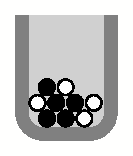
\includegraphics[width=16mm]{img/Urne.pdf}
\end{minipage}\pause

\parspace
Es sei $X(\omega)\in\{0,1\}$ das Ergebnis der Ziehung, wobei $0$ für
\emph{schwarz}, und $1$ für \emph{weiß} stehe. Die Gesamtzahl
der Kugeln ist $s+w$. Für eine schwarze Kugel sind davon $s$ günstig,
für eine weiße sind es $w$. Man erhält somit
\begin{align*}
P(X=0) = \frac{s}{s+w},\\
P(X=1) = \frac{w}{s+w}.
\end{align*}\pause
Wir fassen die beiden Fälle zusammen zu
\[P(X=x) = \frac{(1-x)s+xw}{s+w}.\]
\end{frame}

\begin{frame}
\centerheadline{Ein unbekannter Parameter}
\end{frame}

\begin{frame}
Die Zahl $w$ der weißen Kugeln sei nun unbekannt, entstamme aber aus
dem Bereich $\{0,\ldots,N-1\}$. Zumindest tun wir so, vergleichen
später mit der wahren Zahl. Wir wollen $w$ durch eine Ziehung aus der
Urne schätzen.\pause

\parspace
Dazu sei $W$ die Zufallsgröße für die Zahl der weißen Kugeln.
Wir nehmen zu Anfang an, jede Zahl $w$ wäre gleich wahrscheinlich, also
$P(W=w)=\frac{1}{N}$ für jedes $w\in\{0,\ldots,N-1\}$.\pause

\parspace
Es wird eine Kugel aus der Urne gezogen, was die Evidenz $E:=\{X=x\}$
zu festem $x=0$ oder $x=1$ schafft.
\end{frame}

\begin{frame}
Dem Satz von Bayes nach gilt nun
\[P(W=w\mid E) = \frac{P(E\mid W=w)}{P(E)}P(W=w).\]\pause
Die Terme besitzen hierbei die folgende Bedeutung:

\parspace
\begin{tabular}{@{\qquad}r@{\;\;}c@{\;\;}l}
$P(W=w)$ & --- & \emph{A-priori-Wahrscheinlichkeit}\\[3pt]
$P(W=w\mid E)$ & --- & \emph{A-posteriori-Wahrscheinlichkeit}\\[3pt]
$\frac{P(E\mid W=w)}{P(E)}$ & --- & \emph{Aktualisierungsfaktor}\\[3pt]
$P(E\mid W=w)$ & --- & \emph{Likelihood}
\end{tabular}\pause

\parspace
Zur Bestimmung der A"=posteriori"=Wahrscheinlichkeit benötigen wir den
Aktualisierungsfaktor.
\end{frame}

\begin{frame}
Die Likelihood ist bei
Erhalt der Evidenz bekannt, da sie aufgrund der Bedingung $W=w$ die
übliche Wahrscheinlichkeit der Ziehung aus der Urne bei Kenntnis
des Parameters $w$ ist. Das heißt,
\[P(X=x\mid W=w) = \frac{(1-x)s+xw}{s+w}.\]
\end{frame}

\begin{frame}
Aber wie bestimmen wir $P(X=x)$?\pause

\parspace
Diese ergibt sich mit dem Gesetz der totalen Wahrscheinlichkeit zu
\[P(X=x) = \sum_{k=0}^{N-1}P(X=x\mid W=k)P(W=k),\]
lässt sich also auf die Likelihood und die A"=priori"=Wahrscheinlichkeit
zurückführen, die beide bekannt sind.\pause

\parspace
Wir erhalten
\[P(X=x) = \frac{1}{N}\sum_{k=0}^{N-1}\frac{(1-x)s+xk}{s+k}.\]
\end{frame}

\begin{frame}
Die A"=posteriori"=Wahrscheinlichkeit bestimmt sich also zu
\[P(W=w\mid X=x) = \frac{\frac{(1-x)s+xw}{s+w}}{\sum_{k=0}^{N-1}\frac{(1-x)s+xk}{s+k}}.\]
\end{frame}

\begin{frame}
\centerheadline{Mehrere Stichproben}
\end{frame}

\begin{frame}
Nun würden wir das Updaten der Wahrscheinlichkeit mit einer weiteren
Stichprobe gerne abermals durchführen. Das Setting soll dabei natürlich
unmodifiziert bleiben. Nach der jeweiligen Ziehung wird die Kugel also
wieder zurück in die Urne gelegt, und diese daraufhin wieder gut gemischt.\pause

\parspace
Wir setzen dafür $X=(X_1,\ldots,X_n)$, wobei ein $x=(x_1,\ldots,x_n)$
aus den Stichproben $x_i\in\{0,1\}$ besteht. Die $X_i$ sind unter $W=w$
unabhängig und identisch verteilt. Was unser ursprüngliches $x$ war,
ist nun $x_1$.\pause

\parspace
Bestimmt wurde bislang also nur $P(W=w\mid X_1=x_1)$. Als nächtes kommt
$P(W=w\mid X_1=x_1, X_2=x_2)$. Oder besser gesagt, wir würden letztlich gern
\[P(W=w\mid X=x) = P(W=w\mid X_1=x_1,\ldots, X_n=x_n)\]
bestimmen.
\end{frame}

\begin{frame}
Dem Satz von Bayes nach rechnen wir
\[P(W=w\mid E_2) = \frac{P(E_2\mid W=w)}{P(E_2)}P(W=w)\]
mit $E_2 := \{X_1=x_1,X_2=x_2\} = \{X_1=x_1\}\cap\{X_2=x_2\}$.\pause

\parspace
Aufgrund der stochastischen Unabhängigkeit der $X_i$ bei $W=w$ gilt
\[P(E_2\mid W=w) = P(X_2=x_2\mid W=w)P(X_1=x_1\mid W=w)\]
denn für unabhängige Ereignisse $A,B$ gilt $P(A\cap B)=P(A)P(B)$.
\end{frame}

\begin{frame}
Wir dürfen allerdings nicht einfach $P(E_2)=P(X_1=x_1)P(X_2=x_2)$
rechnen, da $X_1,X_2$ nicht unabhängig sein müssen, weil die Verteilung
von $W$ in ihre Verteilungen eingeht. Wir nutzen daher zuerst das Gesetz
der totalen Wahrscheinlichkeit, zerlegen $P(E_2\mid W=k)$ daraufhin ins
Produkt. Das macht
\begin{align*}
P(E_2) &= \sum_{k=0}^{N-1}P(E_2\mid W=k)P(W=k)\\
&= \sum_{k=0}^{N-1} P(X_2=x_2\mid W=k)P(X_1=x_1\mid W=k)P(W=k).
\end{align*}\pause
Die hinteren Faktoren des Summanden formen wir jetzt um vermittels
\[P(X_1=x_1\mid W=k) = \frac{P(W=k\mid X_1=x_1)}{P(W=k)}P(X_1=x_1).\]
Der Faktor $P(X_1=x_1)$ hängt nicht von $k$ ab, darf also aus der Summe
ausgeklammert werden.
\end{frame}

\begin{frame}
Somit findet sich
\[P(W=w\mid E_2) = \tfrac{P(X_2=x_2\mid W=w)}{\sum_{k=0}^{N-1} P(X_2=x_2\mid W=k)P(W=k\mid X_1=x_1)}\underbrace{\tfrac{P(X_1=x_1\mid W=w)}{P(X_1=x_1)}P(W=w)}_{P(W=w\mid X_1=x_1)}.\]\pause
Wir führen die Aktualisierungen also sequentiell aus, wobei die
aktualisierte Wahrscheinlichkeit $P(W=w\mid X_1=x_1)$ in der zweiten
Aktualisierung die Rolle der A"=priori"=Wahrscheinlichkeit einnimmt.\pause

\parspace
Salopp gesprochen dürfen wir die ursprüngliche A"=priori"=Wahrscheinlichkeit
nach der Aktualisierung verwerfen, und so tun, als wäre die aktualisierte
die vorliegende A"=priori"=Wahrscheinlichkeit.\pause

\parspace
Zu beachten ist hier, dass die Wahrscheinlichkeit zu \emph{jedem} $w$ bestimmt
werden muss. Wir berechnen also nicht eine einzelne Wahrscheinlichkeit, sondern
die gesamte Wahrscheinlichkeitsfunktion $w\mapsto P(W=w\mid X_1=x_1)$,
und daraufhin $w\mapsto P(W=w\mid E_2)$.
\end{frame}

\begin{frame}
Bezüglich $E_0:=\Omega$ und $E_i:=\{X_i=x_i\}\cap E_{i-1}$ ergibt sich also die Rekurrenz
\[P(W=w\mid E_i) = \frac{P(X_i=x_i\mid W=w)}{\sum_{k=0}^{N-1}
P(X_i=x_i\mid W=k)P(W=k\mid E_{i-1})}P(W=w\mid E_{i-1}).\]
\end{frame}

\begin{frame}
\centerheadline{Nochmals mehrere Stichproben}
\end{frame}

\begin{frame}
Nun verhält es sich aber auch so, dass die Summe $Y=\sum_{i=1}^n X_i$
die Zufallsgröße des n"=stufigen Bernoulli"=Experiments darstellt.
Alternativ lässt sich zur Abschätzung also auch der Ansatz
\[P(W=w\mid Y=y) = \frac{P(Y=y\mid W=w)}{P(Y=y)}P(W=w)\]
machen, wobei
\[y\mapsto P(Y=y\mid W=w) = \binom{n}{y}p^y(1-p)^{n-y}\]
mit $p=\frac{w}{s+w}$ die Wahrscheinlichkeitsfunktion der
Binomialverteilung ist.
\end{frame}

\begin{frame}
Nach Entfaltung der totalen Wahrscheinlichkeit im Nenner kürzt
sich der Faktor $\binom{n}{y}$ heraus. Das macht
\[P(W=w\mid Y=y) = \frac{p^y(1-p)^{n-y}P(W=w)}{
\sum_{k=0}^{N-1}p_k^y(1-p_k)^{n-y}P(W=k)}\]
mit $p=\frac{w}{s+w}$ und $p_k = \frac{k}{s+k}$.
\end{frame}

\begin{frame}
Es tut sich die Frage auf, welcher der beiden Ansätze besser schätzt.\pause

\parspace
Die Antwort darauf lautet \emph{keiner}.\pause

\parspace
Beide Rechnungen führen -- Spitzfindigkeiten zur numerischen Güte
beiseitegelassen -- exakt zum selben Resultat.
\end{frame}

\begin{frame}
\centerheadline{Ein paar Begrifflichkeiten}
\end{frame}

\begin{frame}
Wir haben einen \emph{Parameter} $\theta\in\Theta$. Hier ist dies
$\theta:=w$. Als \emph{Parameterraum} haben wir $\Theta:=\{0,\ldots,N-1\}$.
Das Maß $P_\theta$ hängt von diesen Parameter ab. Dies ist hier
\[P_\theta(X=x) = \frac{(1-x)s+x\theta}{s+\theta}.\]\pause
Man nennt
\[L_x\colon\Theta\to [0,1],\quad L_x(\theta) := P_\theta(X=x)\]
die \emph{Likelihood-Funktion}.\pause

\parspace
Da der wahre Parameter $\theta$ unbekannt ist, ermitteln wir unsere
Schätzung für diesen durch eine Zufallsgröße $T(x)$, die man die
\emph{Schätzfunktion} für $\theta$ nennt. Sie ordnet jedem
Stichprobenvektor $x$ einen Schätzwert $t=T(x)$ zu, wobei wir uns
$t\approx\theta$ wünschen.
\end{frame}

\begin{frame}
Wir können $T(x)$ als Erwartungswert der A"=posteriori"=Verteilung
ansetzen.\pause

\parspace
Bezeichnet $p(\theta)$ die
Wahrscheinlichkeitsfunktion der A"=priori- und $p(\theta\mid x)$ die der
A"=posteriori"=Verteilung, haben wir also
\[T(x) := \sum_{\theta\in\Theta}\theta p(\theta\mid x)\]
mit der Bayes-Rechnung
\[p(\theta\mid x) := \frac{L_x(\theta)}{\sum_{t\in\Theta}L_x(t)p(t)} p(\theta)\]
bezüglich $p(\theta):=\frac{1}{|\Theta|}$.
\end{frame}

\begin{frame}
\centerheadline{Frequentistische Deutung}
\end{frame}

\begin{frame}
Bei $P(W=w\mid X=x)$ blieb bislang vage, welche Bedeutung $W$
zukommt. Wir gehen von einer unbekannten wahren Anzahl weißer Kugeln
aus, die geschätzt werden soll. Es tut sich die Frage auf, wo hierbei
der Zufall liegen soll, da es sich bei $W$ um eine Zufallsgröße handelt,
die definitionsgemäß ein zufälliges Ergebnis auf ein anderes abbildet.\pause

\parspace
Aus subjektivistischer Sicht lautet die Antwort darauf, dass die Verteilung
von $W$ die Unkenntnis der wahren Anzahl beschreibt. Die aktualisierte
Verteilung beschreibt dahingehend die verringerte Unkenntnis unter der
Beobachtung der Stichprobe.\pause

\parspace
Das eigentliche Wesen von $W$ verbleibt dennoch im Halbschatten.
Zur Klärung rücken wir den Sachverhalt in die frequentistische Sicht.
Dieser nimmt dabei die Form eines übergeordneten, zweistufigen
Zufallsexperiments an.
\end{frame}

\begin{frame}
Im ersten Teilexperiment wird unter allen möglichen Urnen, also
allen möglichen Konfigurationen von weißen Kugeln, zufällig eine
ausgewählt. Hierbei sei jede Konfiguration gleich wahrscheinlich.\pause

\parspace
Im zweiten Teilexperiment zieht man $n$ mal mit zurücklegen eine
Kugel aus dieser Urne, um den Stichprobenvektor $x$ zu erhalten.\pause

\parspace
Als adäquate Ergebnismenge bietet sich also
\[\Omega = \{0,\ldots,N-1\}\times\{0,1\}^n\]
an. Die Zufallsgrößen nehmen dahingehend die Rolle der
Projektionen 
\[\begin{array}{c@{}lc@{}l}
W &\colon\Omega\to\{0,\ldots,N-1\}, & W((w,x)) &{} :=w,\\[3pt]
X &\colon\Omega\to\{0,1\}^n, & X((w,x)) &{} :=x.
\end{array}\]
ein.
\end{frame}

\begin{frame}
Alle bisherigen Rechnungen bleiben natürlich unverändert gültig.
Die Wahrscheinlichkeit $P(W=w)$ deutet sich nun als die zur Wahl der
Urne mit $w$ Kugeln. Die Likelihood $P(X=x\mid W=w)$ deutet sich
als die Übergangswahrscheinlichkeit unter dieser Urne, so dass
\[P(X=x, W=w) = P(X=x\mid W=w)P(W=w).\]
Insofern die gesuchte Wahrscheinlichkeit $P(W=w\mid X=x)$ allerdings
nicht direkt am Baumdiagramm ablesbar ist, muss sie über die erläuterte
Bayes"=Rechnung bestimmt werden.\pause

\parspace
Darüber hinaus ist der Sachverhalt nun einer Simulation zugänglich.
Wir führen das Experiment eine große Zahl, sagen wir eine Mio. mal durch.
Aus den Ergebnissen $\omega\in\Omega$ werden diejenigen mit $X(\omega)=x$
zu einem fest gewählten $x$ ausgesondert, deren Anzahl sei $H_x$. Zu
einem festen $w$ zählt man nun, wie häufig $X(\omega)=w$ darin
vorkommt, dies sei $H_{xw}$. Man hat nun
\[P(W=w\mid X=x)\approx\frac{H_{xw}}{H_x},\;\text{sofern $H_x\ne 0$}.\]
\end{frame}

\begin{frame}
Sind $X_1,X_2$ nun wirklich stochastisch abhängig? Betrachten wir dazu
die Situation $s:=1$, $N:=2$, $n:=2$. Schon ein Gegenbeispiel $(x_1,x_2)$
mit
\[P(X_1=x_1,X_2=x_2)\ne P(X_1=x_1)P(X_2=x_2)\]
genügt zur Widerlegung der Unabhängigkeit.

\begin{center}
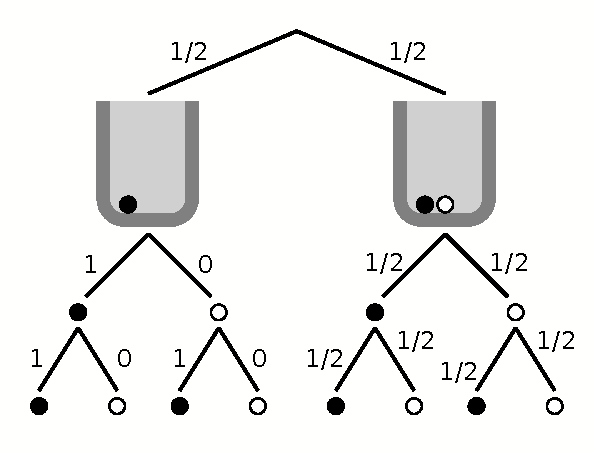
\includegraphics[width=60mm]{img/Urnen22.pdf}
\end{center}
\end{frame}

\begin{frame}
Für jedes $i$ gilt die Rechnung
\[P(X_i=1) = \sum_{k=0}^1 P(X_i=1\mid W=k)W(W=k) =
0\cdot\tfrac{1}{2} + \tfrac{1}{2}\cdot\tfrac{1}{2} = \tfrac{1}{4},\]
womit $P(X_1=1)P(X_2=1)=\tfrac{1}{4}\cdot\tfrac{1}{4}=\tfrac{1}{16}$.\pause

\parspace
Fürs gemeinsame Ereignis $\{X_1=1,X_2=1\}$ ergibt sich allerdings
\begin{align*}
P(X_1=1,X_2=1) &= \sum_{k=0}^1 P(X_1=1,X_2=1\mid W=k)P(W=k)\\
&= \sum_{k=0}^1 P(X_1=1\mid W=k)P(X_2=1\mid W=k)P(W=k)\\
&= 0\cdot 0\cdot\tfrac{1}{2} + \tfrac{1}{2}\cdot\tfrac{1}{2}\cdot\tfrac{1}{2}
= \tfrac{1}{8}.
\end{align*}\pause
Mit $P(X_1=1,X_2=1)=\tfrac{1}{8}\ne\tfrac{1}{16}=P(X_1=1)P(X_2=1)$
liegt also ein Gegenbeispiel zur stochastischen Unabhängigkeit von
$X_1,X_2$ vor.
\end{frame}

\begin{frame}
Ende.
\vfill\hfill\modest{Juli 2025}\\
\hfill\modest{Creative Commons CC0 1.0}
\end{frame}

\end{document}
